\documentclass{article}

\usepackage{url}
\usepackage{hyperref}

\usepackage{graphicx}
\usepackage{subcaption}

\begin{document}
\title{Detectia automata a speciilor invazive in imagini}
\author{Stefan Sebastian \and Zsisku Mihai}
\date{\today}
\maketitle

\newpage

\tableofcontents

\newpage

\section{Introducere}
O specie de animal sau planta introdusa intr-un mediu nou fata de cel in care a evoluat este invaziva daca se inmulteste intr-un ritm rapid si afecteaza mediul in mod negativ, distrugand habitate sau decimand specii locale\cite{WEBSITE:1}.
 
De exemplu, insecta Adelges tsugae, originara din Asia, a dus la uciderea a pana la 80\% din coniferele din specia Tsuga, din unele parti din America de Nord\cite{WEBSITE:2}. In 1946, 20 de castori au fost adusi pe o insula de langa Argentina pentru a fi vanati pentru blana lor. Acestia s-au inmultit si s-au raspandit pe continent si pe insulele din jur. Copacii din zona nu sunt adaptati la activitatea castorilor si majoritatea nu mai cresc dupa ce sunt rosi de acestia. De asemenea castorii creeaza corpuri de apa statatoare care altereaza ciclul nutrientilor din paduri\cite{WEBSITE:3}. Unele specii, precum Scoica Zebra, pot aduce si costuri economice. Acestea blocheaza centrale electrice si instalatii de tratare a apei iar inlaturarea lor din Marile Lacuri(America de Nord) costa aproximativ 500mil\$ anual\cite{WEBSITE:5}.

Pentru identificarea unei astfel de specii este nevoie de specialisti care sa se deplaseze pe teren si sa noteze speciile prezente. O astfel de abordare este scumpa (e nevoie de un numar mare de oameni pregatiti) si ineficienta (oamenii nu pot acoperi zone foarte mari).

Solutia pe care o propunem este identificarea automata a speciilor invazive din imagini. Aceste imagini pot fi capturate automat de camere montate in anumite zone si detectia speciilor invazive se poate face automat, fara nevoie de asistenta umana. Totusi, este necesar un set de date cuprinzator (cateva mii de imagini).

In cadrul acestui experiment am incercat sa clasificam imagini cu Hydrangea. Aceasta planta a fost identificata ca fiind invaziva in Brazilia (sursa imaginilor) si in Macaronesia (4 arhipelaguri de langa Europa si Africa)\cite{BOOK:1}.

\section{Abordari inrudite}

\subsection{CNN}
In articolul Invasive Species Monitoring using Machine Learning\cite{WEBSITE:4} este prezentata o metoda ce obtine 95\% acuratete.  Pentru prelucrarea datelor este folosita tehnica de ‘Contrast Stretching’ care imbunatateste contrastul. Setul de date este extins prin generarea de imagini din setul initial rotite vertical, la care se adauga padding si sunt redimensionate prin interpolare liniara. Modelul folosit este o Retea Neuronala Convolutiva cu 11 straturi si functia de activare ReLU.

\subsection{Ansamblu ResNet + VGG}
In articolul Invasive Species Detection\cite{ARTICLE:1} se foloseste un ansamblu din modele modificate de ResNet si VGG pentru a obtine o acuratete de 99.36\%. ResNet, Residual Networks, este o arhitectura dezvoltata de o echipa de cercetatori de la Microsoft proiectata pentru a preveni problema ‘Vanishing Gradient’, a neuronilor care ‘mor’ in antrenament si devin inutili. Se foloseste de conexiuni reziduale pentru a transfera informatie intre straturi\cite{ARTICLE:2}. VGG este o arhitectura care foloseste doar convolutii de 3x3 si pooling de 2x2 si tinde sa aiba o adancime mai mare\cite{ARTICLE:3}.
 
In aceasta lucrare a fost folosita metoda ‘transfer learning’ care presupune preluarea unor modele deja antrenate, in acest caz VGG si ResNet pe baza de date ImageNet, si inlocuirea ultimului strat pentru a se potrivi cu problema curenta. Dimensiunea imaginilor a fost redusa la 224x224 folosind scalarea Lanczos, o tehnica mai lenta dar care mentine calitatea mult mai bine in comparatie cu alte metode. Cele mai bune rezultate le-au obtinut prin ansamblul: VGG13, ResNet(18, 34, 50, 101, 152), folosind media probabilitatilor fiecarui model pentru fiecare imagine si alegand pe cea mai mare. Numerele asociate modelelor reprezinta numarul de straturi folosite.

\subsection{Transfer learning de la VGG16}
In Visual Classifier for Invasive Plant Species\cite{ARTICLE:4} s-au folosit diferite modele bazate pe retele neuronale convolutive preantrenate VGG16, s-a incercat augmentarea setului de date folosind translatii verticale, orizontale, modificarea contrastului, etc. VGG16 este o retea preantrenata pentru a extrage trasaturi (feature-uri). Dupa aceasta retea s-au adaugat 2-3 straturi complet conectate (fully connected). Pentru a preveni alterarea majora a retelei VGG16, s-a folosit Stochastic Gradient Descent, cu o rata mica de invatare. S-a folosit functia de activare ReLU. Ca masura a rezultatului modelului s-a folosit AUROC (“Area Under the Receiver Operating Characteristic curve“). S-a observat ca prin augmentarea datelor performanta modelelor a scazut, posibil din cauza zgomotului introdus de procesele de augmentare.

\section{Metoda de lucru}

\subsection{Invatare nesupervizata din informatii extrase de autoencoders}
Primul pas consta in prelucrarea imaginilor de antrenament prin redimensionare sau convertire la alb-negru. Aceste imagini sunt folosite apoi pentru a antrena un autoencoder.

Un autoencoder este o retea neurala care seteaza valoarea de iesire ca fiind egala cu cea de intrare, deci incearca sa invete functia de identitate. Prin setarea unor constrangeri (dimensiuni reduse) algoritmul poate invata anumite caracteristici ale datelor\cite{BOOK:2}. In aceasta abordare am folosit un autoencoder bazat pe retele convolutive, format din mai multe straturi de convolutie, maxpooling si upsampling dispuse in ‘oglinda’. Modelul de codificare este un strat intermediar al autoencoderului.

Modelul invatat de autoencoder e folosit pentru a extrage reprezentarea codificata a imaginilor, fiecare tablou extras de CNN reprezentand o caracteristica(feature). Aceste caracteristici sunt combinate intr-un singur tablou si folosite ca date de intrare pentru un algoritm de clusterizare (K-Means). Pentru a stabili daca etichetele generate de algoritmul nesupervizat corespund celor atasate imaginilor am comparat rezultatele cu un set de imagini de referinta alese de mana.

\section{Setul de date}
Pentru acest proiect am folosit setul de date aferent competitiei Invasive Species Monitoring\cite{WEBSITE:6} de pe Kaggle. Acesta consta din 2295 de imagini etichetate manual. Imaginile au fost facute intr-o padure din Brazilia si o parte din ele contin specia invaziva Hydrangea. 1448 de imagini din setul total contin Hydrangea, deci 63\% din exemple sunt pozitive. Toate imaginile sunt color si au dimensiunea 866x1154 pixeli. Majoritatea imaginilor pozitive contin tufe de Hydrangea in centrul imaginii. Imaginile negative contin scene din padure, iar in unele apar lacuri sau oameni.Un exemplu de imagine pozitiva si negativa poate fi vazut in \ref{fig:posneg}.

\begin{figure}[h!]
  \centering
  \begin{subfigure}[b]{0.4\linewidth}
    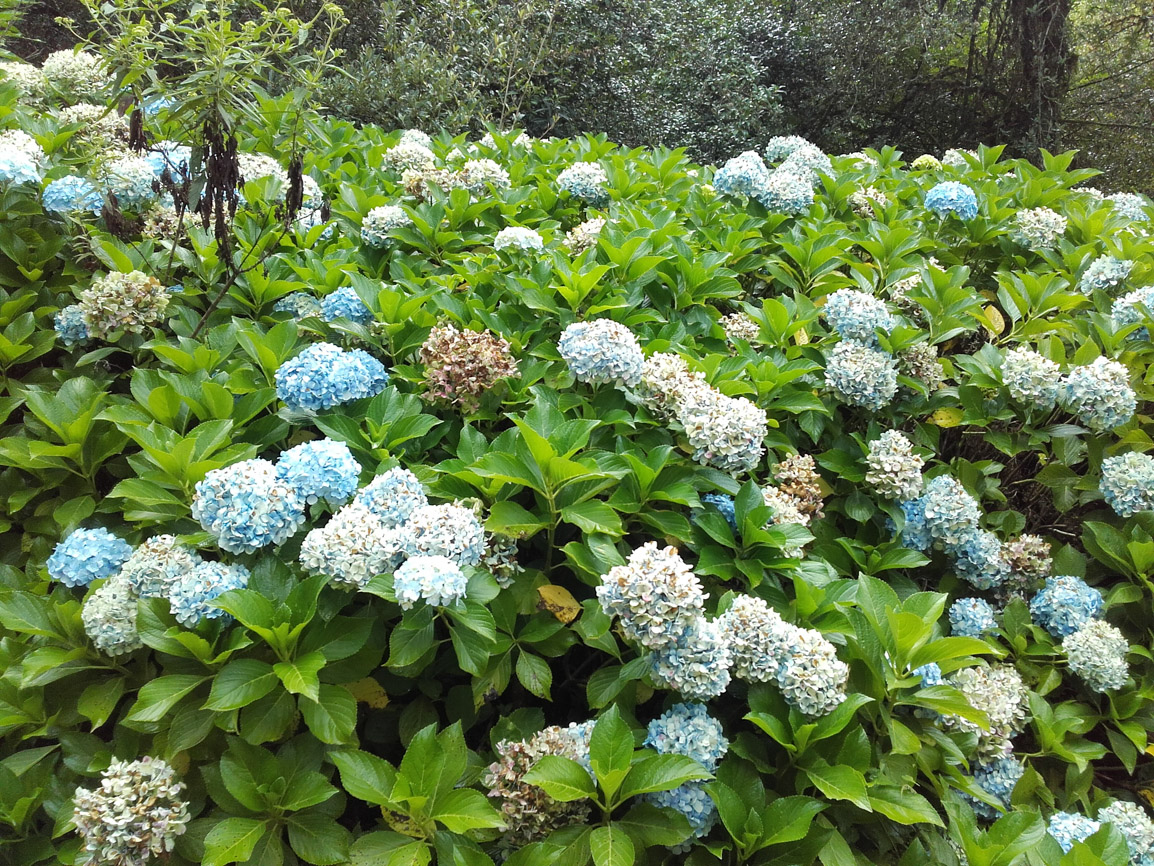
\includegraphics[width=\linewidth]{pos.jpg}
    \caption{Tufa de Hydrangea.}
  \end{subfigure}
  \begin{subfigure}[b]{0.4\linewidth}
    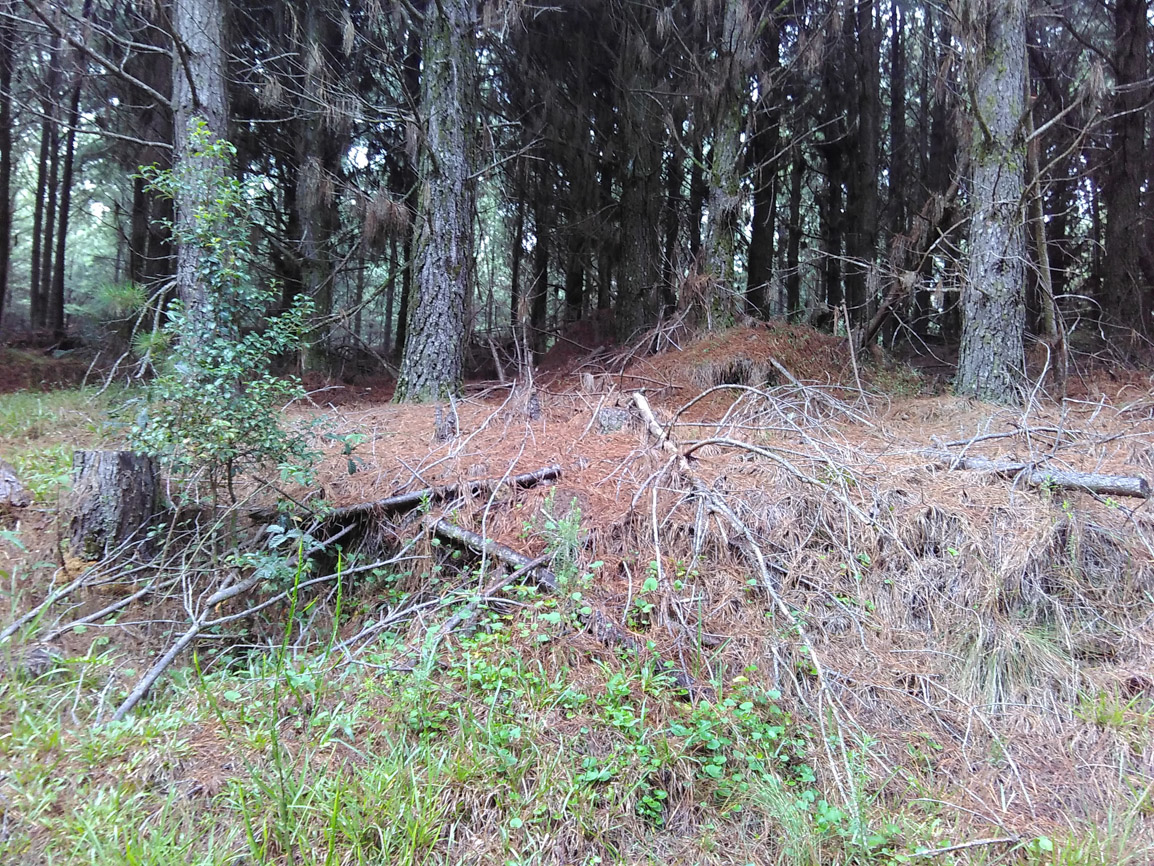
\includegraphics[width=\linewidth]{neg.jpg}
    \caption{Imagine din padure.}
  \end{subfigure}
  \caption{Exemplu imagini pozitive si negative.}
  \label{fig:posneg}
\end{figure}


\section{Parametraj algoritmi}

\subsection{Abordarea 1}

In primul rand am incercat sa determin cea mai potrivita arhitectura pentru autoencoder. Am rulat mai multe experimente, cu 1, 3 si 4 straturi de convolutie in modelul de codificare. Am observat ca acuratetea nu variaza foarte mult, deci am ales sa folosesc un singur strat de convolutie pentru simplitate.\ref{tab:arh}

\begin{table}[h!]
  \begin{center}
    \caption{Arhitectura autoencoder}
    \label{tab:arh}
    \begin{tabular}{c|c|c|c|c}
      \textbf{ConvolutionLayers} & \textbf{Epochs} & \textbf{BatchSize} & \textbf{EncodingLoss} & \textbf{Accuracy}\\
      \hline
      4 & 50 & 20 & 0.62 & 54\% \\
      1 & 50 & 20 & 0.59 & 56\% \\
      3 & 50 & 20 & 0.6 & 54\%  \\
      1 & 50 & 50 & 0.58 & 55\% \\
      \end{tabular}
  \end{center}
\end{table}

\newpage
\bibliography{bibliografie} 
\bibliographystyle{ieeetr}

\end{document}